Um artes�o possui potes cil�ndricos de tinta cuJas medidas externas s�o 4 cm de di�metro e 6 cm de altura. Ele pretende adquirir caixas organizadoras para armazenar seus potes de tinta, empilhados verticalmente com tampas voltadas para cima, de forma que as caixas possam ser fechadas. 
No mercado, existem cinco op��es de caixas organizadoras, com tampa, em formato de paralelep�pedo reto ret�ngulo, vendidas pelo mesmo pre�o, possuindo as seguintes dimens�es internas: 

\begin{figure}[h]
\centering
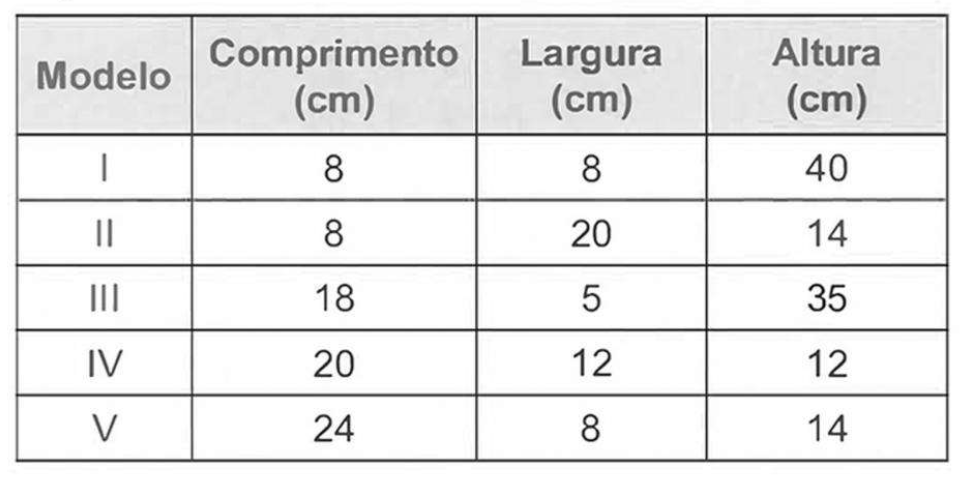
\includegraphics[width=8cm]{../figuras/q150-2018.png}
\end{figure}

Qual desses modelos o artes�o deve adquirir para conseguir armazenar o maior n�mero de potes por caixa?

\begin{enumerate}
\item[a)]I
\item[b)]II
\item[c)]III
\item[d)]IV
\item[e)]V
\end{enumerate}